% Settings for the default beamer theme
\documentclass[english, aspectratio=169]{beamer}
\usepackage[T1]{fontenc}
\usepackage[utf8]{inputenc}
\usepackage{tabularx}
\usepackage{babel}
\usepackage[ruled,vlined]{algorithm2e}
\SetAlgorithmName{Algoritmus}{algoritmus}{List of Algorithms}
\setcounter{secnumdepth}{3}
\setcounter{tocdepth}{3}

\makeatletter

\newcommand\makebeamertitle{\frame{\maketitle}}

% (ERT) argument for the TOC
\AtBeginDocument{%
  \let\origtableofcontents=\tableofcontents
  \def\tableofcontents{\@ifnextchar[{\origtableofcontents}{\gobbletableofcontents}}
  \def\gobbletableofcontents#1{\origtableofcontents}
}

% Theme settings
\usetheme{Frankfurt}
\usecolortheme{default}
\usefonttheme[onlymath]{serif}

% Template settings
\setbeamertemplate{navigation symbols}{}
\setbeamertemplate{blocks}[rounded][shadow=false]
\setbeamertemplate{title page}[default][colsep=-4bp, rounded=true, shadow=false]
\makeatother

% Define a custom darker red color
\definecolor{DarkerRed}{RGB}{139,0,0} % Adjust the RGB values as needed

% Use the newly defined color in Beamer theme elements
\setbeamercolor{structure}{fg=DarkerRed} % Changes basic structural elements to Darker Red
\setbeamercolor{title in head/foot}{bg=DarkerRed} % Changes the title in header/footer to Darker Red


\begin{document}

% Title page
\section{Bevezetés}
\title[]{Üzleti Elemzések Módszertana}
\subtitle{8. Előadás: Generatív modellezés}
\author[Kuknyó Dániel]{Kuknyó Dániel\\Budapesti Gazdasági Egyetem}
\date{2023/24\\2.félév}
\makebeamertitle

% Table of contents slide
\begin{frame}
\tableofcontents{}
\end{frame}

% Table of contents of the current section
\begin{frame}
\tableofcontents[currentsection]
\end{frame}

\begin{frame}{Feltételes valószínűségek}
\begin{columns}
\begin{column}{.5\textwidth}
Valamely $A$ esemény feltételes valószínűsége azt jelenti, mekkora az esély $A$ esemény bekövetkezésére feltéve, hogy $B$ esemény már megtörtént. Ennek jelölése:
\begin{block}{}
\[
P\left( A \vert B \right) = \frac{P\left( A \cap B \right)}{P\left( B \right)}
\]
\end{block}
Ennek megfelelően például az a valószínűség, hogy egy rendelés csalóktól érkezik feltéve, hogy kupont használtak: 
\begin{block}{}
\vspace{-.4cm}
\[
P\left( \text{Csaló} \vert	\text{Kupon} \right) = \frac{P\left( \text{Csaló} \cap \text{Kupon} \right)}{P\left( \text{Kupon} \right)}
\]
\end{block}
\end{column}
\begin{column}{.5\textwidth}
\begin{center}
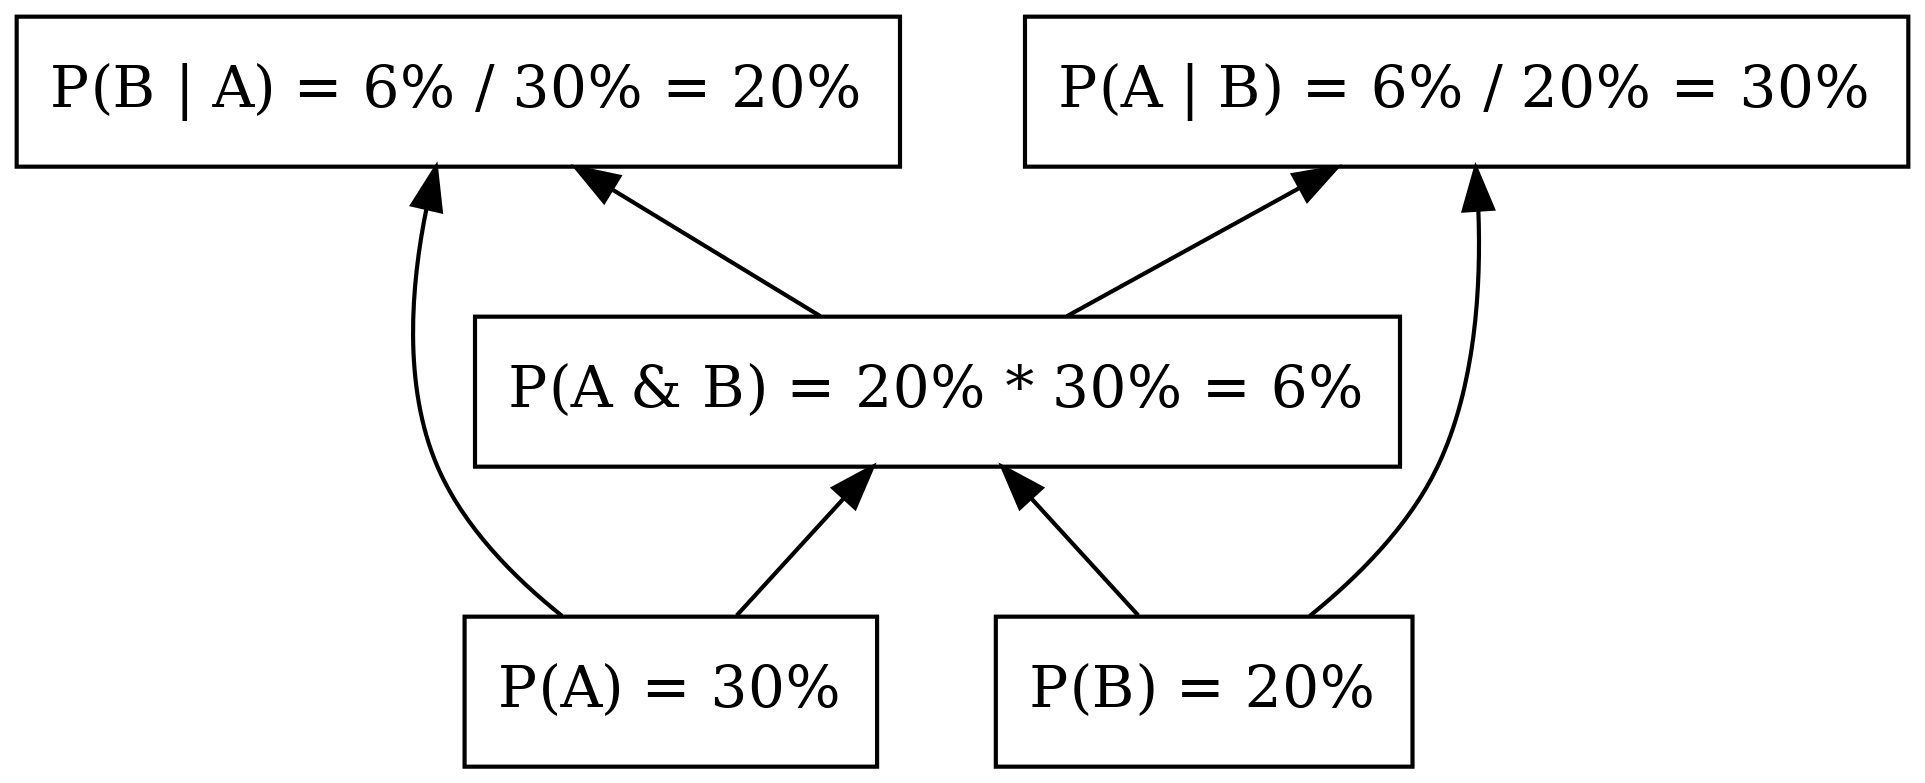
\includegraphics[width=7cm, height=7cm, keepaspectratio]{graphs/generative_1.png}
\end{center}
\end{column}
\end{columns}
\end{frame}

\begin{frame}{Inverz feltételes valószínűségek}
\begin{columns}
\begin{column}{.5\textwidth}
Az inverz feltételes valószínűség kiszámítható a Bayes-tételnek megfelelően a feltételes valószínűség és a nem feltételes valószínűségek segítségével:
\begin{block}{}
\[
P\left( B \vert A \right) = \frac{P\left( A \vert B \right) P\left( B \right)}{P\left( A \right)}
\]
\end{block}
A probabilisztikus modellek ezt veszik alapul. A probabilisztikus osztályozás célja valamely $\mathcal{L}$ címkehalmaz valószínűségét megbecsülni adott $x$ változóhalmaz alapján:
\begin{block}{}
\[
P\left( \mathcal{L} \vert x \right) = \frac{P\left( x \vert \mathcal{L} \right)P\left( \mathcal{L} \right)}{P\left( x \right)}
\]
\end{block}
\end{column}
\begin{column}{.5\textwidth}

\end{column}
\end{columns}
\end{frame}

\end{document}


























